\problemname{Chaotic Construction}

\newcommand{\cityname}[0]{Gircle}
\newcommand{\citynamefat}[0]{\textbf{G}ircle}
\newcommand{\citynameemph}[0]{\emph{Gircle}}


The city \cityname{} has only one street, and that street is cyclic.
This was very convenient in times when people didn't carry a device with
compass, GPS and detailed maps around in their pockets,
because you only have to walk in one direction and will certainly
arrive at your destination.
Since \cityname{}'s founding a lot of time has passed. Civil
engineers now know a lot more about road network design and most people have
immediate access to reliable and accurate navigation systems.
However, the passage of time also affected the old street surface and more and more
cracks and potholes appeared.

The local government has finally decided to improve the situation, but
preserving the city's historic appeal and building new streets are unfortunately mutually exclusive.
Because tourism is vital for \cityname{}'s economy, the government's only viable option for improving the situation is to renovate segments of the street when necessary.
\cityname{}'s street is very narrow, so a construction site at a street
segment makes it impossible for citizens to pass that segment or even leave or enter it.

As a member of the \citynameemph{} \emph{Construction and Planning Commission} (GCPC), you always know when one of the $n$ street segments
is closed or reopened.
Naturally, the citizens expect you to tell them whether the trips they
want to do are currently possible.

\begin{figure}[h]
	\centering
	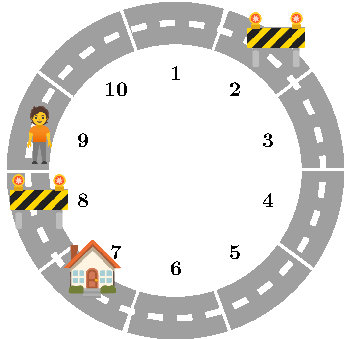
\includegraphics[width=0.45\textwidth]{image}
	\caption{Depiction of the query ``\texttt{?~9 7}'' in the sample input.}
\end{figure}

\begin{Input}
	The input consists of:
	\begin{itemize}
	  \item One line with two integers $n$ ($2 \leq n \leq 10^5$) and $q$ ($1
		  \leq q \leq 10^5$), the number of street segments and the number of events. No street segment is initially closed.
	  \item $q$ lines, each describing an event. Each event is described in one of the following ways:
	  \begin{itemize}
		  \item ``\texttt{- a}'': Segment $a$ ($1 \leq a \leq n$) is closed. It is guaranteed that segment $a$ was open before.
		  \item ``\texttt{+ a}'': Segment $a$ ($1 \leq a \leq n$) is reopened. It is guaranteed that segment $a$ was closed before.
	    \item ``\texttt{?~a b}'': A person asks you if it is possible to go from segment $a$ to segment $b$ ($1 \leq a, b \leq n \text{ and } a\neq b$).
	  \end{itemize}
	\end{itemize}
\end{Input}

\begin{Output}
For each event of the form ``\texttt{?~a b}'', print one line containing the word ``\texttt{possible}'', if it is possible to move from segment $a$ to segment $b$, or ``\texttt{impossible}'' otherwise.
If $a$ or $b$ are currently closed, the answer is ``\texttt{impossible}''.
\end{Output}
